\documentclass[11pt, a4paper, leqno]{article}
\usepackage{a4wide}
\usepackage[T1]{fontenc}
\usepackage[utf8]{inputenc}
\usepackage{float, afterpage, rotating, graphicx}
\usepackage{epstopdf}
\usepackage{longtable, booktabs, tabularx}
\usepackage{fancyvrb, moreverb, relsize}
\usepackage{eurosym, calc}
% \usepackage{chngcntr}
\usepackage{amsmath, amssymb, amsfonts, amsthm, bm}
\usepackage{caption}
\usepackage{mdwlist}
\usepackage{xfrac}
\usepackage{setspace}
\usepackage{xcolor}
\usepackage{subcaption}
\usepackage{minibox}
% \usepackage{pdf14} % Enable for Manuscriptcentral -- can't handle pdf 1.5
% \usepackage{endfloat} % Enable to move tables / figures to the end. Useful for some submissions.


\usepackage[
    natbib=true,
    bibencoding=inputenc,
    bibstyle=authoryear-ibid,
    citestyle=authoryear-comp,
    maxcitenames=3,
    maxbibnames=10,
    useprefix=false,
    sortcites=true,
    backend=biber
]{biblatex}
\AtBeginDocument{\toggletrue{blx@useprefix}}
\AtBeginBibliography{\togglefalse{blx@useprefix}}
\setlength{\bibitemsep}{1.5ex}
\addbibresource{refs.bib}





\usepackage[unicode=true]{hyperref}
\hypersetup{
    colorlinks=true,
    linkcolor=black,
    anchorcolor=black,
    citecolor=black,
    filecolor=black,
    menucolor=black,
    runcolor=black,
    urlcolor=black
}


\widowpenalty=10000
\clubpenalty=10000

\setlength{\parskip}{1ex}
\setlength{\parindent}{0ex}
\setstretch{1.5}


\begin{document}

\title{Skills and Wages\thanks{Poooja Bansal, University of Bonn. Email: \href{mailto:pooja.bansal2610@gmail.com}{\nolinkurl{pooja [dot] bansal2610 [at] gmail [dot] com}}.}}

\author{Poooja Bansal}

\date{
{\bf Preliminary -- please do not quote} 
\\[1ex] 
\today
}

\maketitle


\begin{abstract}
	We provide joint evidence on the relationship between individuals’ cognitive abilities, their personality and earnings for individuals in  Germany using Mincer approach. The paper also estimates the relationships for different categories of occupation defined using the Goldthorpe  classification, 1992. With the data from the German Socio-Economic Panel Study, we employ scores from two short IQ-tests and a set of measures of personality traits which includes items from the Five Factor Personality Inventory. We regress our variables on log hourly wages using different specifications. The results suggest Education and experience are significant factors in the labor market. Our estimates for cognitive abilities indicate no association with wages for any occupations whereas for personality traits, our findings are heterogeneous, varying for different occupations.\\
\\
Keywords: Cognitive skills, Personality traits,SOEP, Occupation, Mincer, Wages \\
\\
Acknowledgement:  We would like to thank Prof.Dr.Thomas Dohmen and Dr.Philipp  Eisenhauer, University of Bonn for providing us with their expertise and guidance during the course of this research.
\end{abstract}
\clearpage

\section{Introduction} % (fold)
\label{sec:introduction}

There has been a growing interest in understanding the effects of non-cognitive skills and personality traits, on labour market outcomes. Many empirical studies have recognized the increasing importance of non-cognitive skills along with the cognitive skills. We try to build on this by studying the effects of both cognitive and non-cognitive skills on individuals’ wage profiles. Since the requirements for these skills vary with different occupations, we investigate the variations  by analyzing how these skills affect the wage profiles of individuals across different occupation levels.\par
The objective of this paper is twofold. We first examine whether cognitive and non-cognitive skills explain difference in hourly wages after controlling for experience and schooling, particularly the relative magnitude of the impact. Secondly we seek to estimate how the skill demands vary across different occupation levels. \par

People typically embody both type of skills: Cognitive skills driving their reasoning and thinking; and non-cognitive skills incorporating their personality traits.
Neisser (1996) defines Cognitive skill as “the ability to understand complex ideas, to adapt effectively to the environment, to learn from experience, to engage in various forms of reasoning, to overcome obstacles by taking thought.” There are numerous studies that have established measurements for cognitive abilities, for instance AFQT scores derived from the Armed Services Vocational Aptitude Battery (ASVAB) , GAT scores test which exists in the Commonwealth nations and IQ performance tests by DIW, Germany. These scores usually approximate cognitive abilities.\par
Most of the literature so far has focused on cognitive abilities only and ignored the importance of non-cognitive skills in labour market analysis due the fallibility of the measures. The skills, popularly known as the personality traits, encompasses many abilities perseverance, patience, reliability, cooperation, emotional stability, self-efficacy, self-esteem and security. Many economists have produced large body of evidence that employers in labor market have recognized the relationship between non-cognitive skills and productivity. This recognition have led to the evolution of measures like  Rosenberg Self esteem scale and Rotter Locus of control, the Big Five Factor Model to study the importance of these in the labor market. \par
The studies so far have discussed the importance of these skills in the labor market. We are contributing to this literature by establishing the relationships between these skills and occupations. But to what extent is occupation useful to understand how education and skills are related with wages. With the rapidly changing trends in the global labor market, employers today want their employees to possess a certain degree of qualification, in terms of skills, education and experience, due to the  non-pecuniary characteristics of different jobs. And in this highly competitive market, employees are keen to develop their qualifications to suit the market needs. Hence we see how these qualifications change in the occupational hierarchy.

This paper continues in the following order: In the next section we will discuss some of the literature which focuses on similar research area that helped us structure our expectations. In the Data section, we describe our data and source. In the Methodology section, we present our econometric framework, followed by the Result section where the first part explains the general relationship of skills for different individuals and then in the second part, we explore the differences in the relationships across various occupational levels. We then provide the robustness checks and finally conclude our analysis.

\section*{Literature Review}

There have been numerous studies which investigated the effect of cognitive skills and personality traits on wages.Heineck and Anger (2008) confirms that employers highly value individuals’ skills. Farkas (1997), Jenkins (2001) also confirm that employers assess cognitive and non-cognitive skills for hiring, promotion and wage setting policies.\par

On one hand, some studies suggested substantial returns to cognitive skills Anger \& Guido Heineck (2005) have established a positive relationship between cognitive skills and labor market outcomes, suggesting that abilities are correlated to the
wages in a significantly positive way for German workers.Murnane, Willett \& Levy (1995) also recognized the importance of cognitive skills in wage determination.While on the other hand, many research works found that cognitive ability has a very little  or no effect on earnings.(Bound et al.(1986)). Also, Cawley, Heckman \& Vytlacil (2001) and  Zax \& Rees (2002) reported that the effect of cognitive skills is much smaller than what has been asserted by previous analyses and is rather a poor estimator of earnings.\par

As for personality traits, attention is growing towards its relationship with labor market. Gintis \& Osborne( 2001) explained how some personality traits matter for employers because they facilitate the production of effort at work and affect labour productivity. 
Heckman,Stixrud \& Urzua (2006) suggested that non-cognitive skill is an equally strong determinant, if not more, as cognitive skill. Bowles \& Gintis (1976) and Edwards (1976) in their work showed that skills such as dependability and persistence are highly valued by employers.\par

However, studies have not sufficiently recognised the role that occupation plays, along with the individuals' skills, in the determination of wages. Beyer\& Knight(1989) studied how wages vary across different occupations in Africa. Birnbaum (1976) interpreted the observed effect of a worker's initial skill category on his current wage. Stewart (1977) found that the British returns to education were generally higher in the non-manual than in the manual occupations and lowest for the unskilled, and that the returns to experience also differed considerably by occupation. Carbonaro (2007) explained that education and cognitive skills are positively related to earnings among workers within narrowly defined occupations.

Overall there is vast literature on the importance of both kinds of skills for wage determination. With our paper, we take a closer look at the wage-skill relationships across different occupational levels.


\section*{Expectations}

With the prior findings from previous empirical studies on non-cognitive and cognitive skills as determinants of labor market outcomes, we were able to set up expectations for the present study. 
In line with the previous research, we expect cognitive skills to have either positive or no association with the earnings. With respect to the personality traits used, we expect no significant relation between Extraversion and wages, a positive relationship for Openness and conscientiousness and negative for Neuroticism and Agreeableness.\par

We believe we are the first one to investigate this skill-wage relationship with respect to occupations using the Goldthorpe classification. So we built our expectations based on our knowledge of the subject.For occupations, we expect cognitive skills to be either positively or not related to the occupational categories. For personality traits, we expect more heterogeneous results for each category of occupation, depending on their work task and roles.


If you are using this template, please cite this item from the references: \citet{GaudeckerEconProjectTemplates}

\citet{Schelling69} example in the code is taken from \citet{StachurskiSargent13}

\section*{Data}

This paper analyzes the data from the German Socio Economic Panel. SOEP is a wide-ranging representative micro-database providing comprehensive socio-economic information on private households in Germany. The panel was first started in 1984 and data for about 12,200 randomly selected respondents, in West Germany, was collected. After German reunification, data for about 4500 respondents, from East Germany, has been added. We use two recent waves which include data on cognitive skills (2005), two short verbal and performance tests, and personality traits (2006), items pertaining to the Big Five Factor model. We retrieved the data for occupation and education from the personal questionnaire of 2005. 

\subsection*{\textit{\underline{Measures of Cognitive skills}}}
The fully fledged IQ tests couldn’t be conducted because of the large scale panel survey.The organization conducted two short tests to evaluate cognitive skills in year 2006. These were: A Word Fluency Test and Symbol Correspondence Test. These tests correspond to modules  of the Wechsler Adult Intelligence Scale (WAIS)\footnote{Wechsler Adult Intelligence Scale (WAIS) comprises 14 modules, seven on verbal IQ and seven on performance IQ (Groth-Marnat, 1997, Kline, 1999)}. 
For the Word Fluency test, which corresponds to the verbal IQ module of WAIS, respondents were asked to name as many animals as possible in 90 seconds and for the Symbol Recognition Test, corresponding to the Performance IQ module, respondents had to match as many number and symbols as possible in 90 seconds using the correspondence list provided to them. We have standardized the test scores since they were measured on different scales.

\subsection*{\textit{\underline{Measures of Non-Cognitive skills}}}

Over time, psychologists have developed a widely accepted personality taxonomy known as the Big Five model which identifies five broad aspects of Personality namely: Openness, Conscientiousness, Extraversion, Agreeableness, and Neuroticism 
(OCEAN). Openness can be defined as a tendency to experience new adventures and emotions, to develop unusual ideas, and to have curiosity. Conscientiousness can be seen as a desire to act in an organized, disciplined, and dutiful manners. Aiming for organized planning instead of spontaneous behaviours. Extraversion can be associated with optimistic behaviours and positive energy, where a person tends to seek attention and interaction in the company of others. Agreeableness can measure if a person is well tempered and cooperative or if he/she is suspicious or untrustworthy. Neuroticism defines the level of emotional stability of a person and can be related to unpleasant emotions such as depression, anger or vulnerability. \par
In 2005, SOEP included questions related to individuals’ personality. The questions are associated to the Big Five Factor model which comprises of the personality aspects described above. Since extensive questioning to generate the scores pertaining to Personality wasn’t feasible in SOEP, the data instead provides us with 15 items\footnote{The items included and the classification is presented in the Appendix Table 1} in which three items apprehends to one personality dimension. The questions were answered on a scale of 1[does not apply] to 7[applies fully]. We have taken averages of the each three items of the respective personality factor of the big five model and standardized them. 

\subsection*{\textit{\underline{Determination of Hourly Wages }}}

SOEP doesn’t collect data on hourly wages directly. Instead it provides data on monthly income from primary employment and actual weekly working hours including overtime. We calculate the hourly wages by dividing the monthly income with the product of weekly hours and the estimated factor of 4.3\footnote{Number of weeks/Number of months = 52/12 = 4.3} for the number of weeks. The measurement errors, possibly existing in working hours or monthly income can influence the results. 

\subsection*{\textit{\underline{Analytical Sample}}}

To address the research question posted in the study, the analytical sample is limited to individuals between age 20 and 60  who were in full time employment, in order to include only those who most likely have completed their education and were below the retirement age. We excluded the observations which had missing values. For individuals reporting zero wages, a small value of 0.0001 was assigned before it was transformed to a logarithmic scale. For categorizing the occupations, we used the  Goldthorpe \footnote{ Goldthorpe class scheme combining occupation categories in light of level of income, economic security, advancement, work authority and responsibility.  
} classification scale.  We have, however,  excluded the category for  agricultural workers and self-employed people due to their very small sample size. The total sample size turned out to be 2581\footnote{The sample size in our analysis rather low since we had to restrict our sample to the  individuals who are SOEP respondents in both 2005 and 2006 and, more limiting, were the CAPI surveyed in 2006 for cognitive skills, since only those were the only potential respondents of the ultra-short IQ-tests.Further, for occupational classification we used the data from the generated variable file which led to a further reduction.}


\begin{figure}
    \caption{Segregation by cycle in the baseline \citet{Schelling69} model as in the \citet{StachurskiSargent13} example}
    
    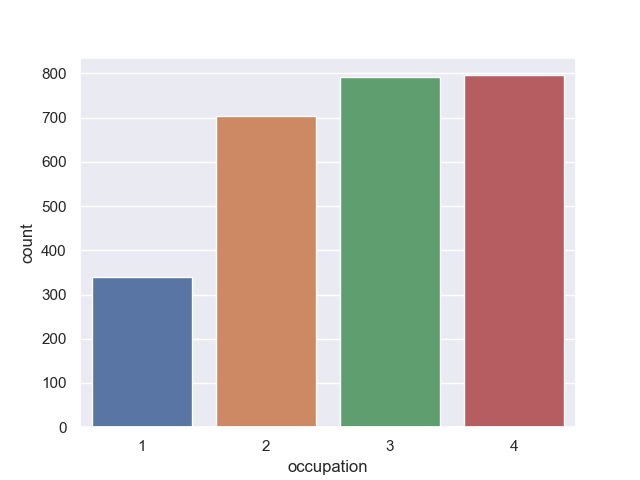
\includegraphics[width=0.5\textwidth]{../../out/figures/occupation_count}

\end{figure}



% section introduction (end)




\setstretch{1}
\printbibliography
\setstretch{1.5}




% \appendix

% The chngctr package is needed for the following lines.
% \counterwithin{table}{section}
% \counterwithin{figure}{section}

\end{document}
